% This contents of this file will be inserted into the _Solutions version of the
% output tex document.  Here's an example:

% If assignment with subquestion (1.a) requires a written response, you will
% find the following flag within this document: <SCPD_SUBMISSION_TAG>_1a
% In this example, you would insert the LaTeX for your solution to (1.a) between
% the <SCPD_SUBMISSION_TAG>_1a flags.  If you also constrain your answer between the
% START_CODE_HERE and END_CODE_HERE flags, your LaTeX will be styled as a
% solution within the final document.

% Please do not use the '<SCPD_SUBMISSION_TAG>' character anywhere within your code.  As expected,
% that will confuse the regular expressions we use to identify your solution.

\def\assignmentnum{2 }
\def\assignmenttitle{XCS330 Problem Set \assignmentnum}

\documentclass{article}
\usepackage[top = 1.0in]{geometry}

\usepackage{graphicx}

\usepackage[utf8]{inputenc}
\usepackage{listings}
\usepackage[dvipsnames]{xcolor}
\usepackage{bm}
\usepackage{algorithm}
\usepackage{algpseudocode}
\usepackage{framed}

\definecolor{codegreen}{rgb}{0,0.6,0}
\definecolor{codegray}{rgb}{0.5,0.5,0.5}
\definecolor{codepurple}{rgb}{0.58,0,0.82}
\definecolor{backcolour}{rgb}{0.95,0.95,0.92}

\lstdefinestyle{mystyle}{
    backgroundcolor=\color{backcolour},   
    commentstyle=\color{codegreen},
    keywordstyle=\color{magenta},
    stringstyle=\color{codepurple},
    basicstyle=\ttfamily\footnotesize,
    breakatwhitespace=false,         
    breaklines=true,                 
    captionpos=b,                    
    keepspaces=true,                 
    numbersep=5pt,                  
    showspaces=false,                
    showstringspaces=false,
    showtabs=false,                  
    tabsize=2
}

\lstset{style=mystyle}

\newcommand{\di}{{d}}
\newcommand{\nexp}{{n}}
\newcommand{\nf}{{p}}
\newcommand{\vcd}{{\textbf{D}}}
\newcommand{\Int}{\mathbb{Z}}
\newcommand\bb{\ensuremath{\mathbf{b}}}
\newcommand\bs{\ensuremath{\mathbf{s}}}
\newcommand\bp{\ensuremath{\mathbf{p}}}
\newcommand{\relu} { \operatorname{ReLU} }
\newcommand{\smx} { \operatorname{softmax} }
\newcommand\bx{\ensuremath{\mathbf{x}}}
\newcommand\bh{\ensuremath{\mathbf{h}}}
\newcommand\bc{\ensuremath{\mathbf{c}}}
\newcommand\bW{\ensuremath{\mathbf{W}}}
\newcommand\by{\ensuremath{\mathbf{y}}}
\newcommand\bo{\ensuremath{\mathbf{o}}}
\newcommand\be{\ensuremath{\mathbf{e}}}
\newcommand\ba{\ensuremath{\mathbf{a}}}
\newcommand\bu{\ensuremath{\mathbf{u}}}
\newcommand\bv{\ensuremath{\mathbf{v}}}
\newcommand\bP{\ensuremath{\mathbf{P}}}
\newcommand\bg{\ensuremath{\mathbf{g}}}
\newcommand\bX{\ensuremath{\mathbf{X}}}
% real numbers R symbol
\newcommand{\Real}{\mathbb{R}}

% encoder hidden
\newcommand{\henc}{\bh^{\text{enc}}}
\newcommand{\hencfw}[1]{\overrightarrow{\henc_{#1}}}
\newcommand{\hencbw}[1]{\overleftarrow{\henc_{#1}}}

% encoder cell
\newcommand{\cenc}{\bc^{\text{enc}}}
\newcommand{\cencfw}[1]{\overrightarrow{\cenc_{#1}}}
\newcommand{\cencbw}[1]{\overleftarrow{\cenc_{#1}}}

% decoder hidden
\newcommand{\hdec}{\bh^{\text{dec}}}

% decoder cell
\newcommand{\cdec}{\bc^{\text{dec}}}

\usepackage[hyperfootnotes=false]{hyperref}
\hypersetup{
  colorlinks=true,
  linkcolor = blue,
  urlcolor  = blue,
  citecolor = blue,
  anchorcolor = blue,
  pdfborderstyle={/S/U/W 1}
}
\usepackage{nccmath}
\usepackage{mathtools}
\usepackage{graphicx,caption}
\usepackage[shortlabels]{enumitem}
\usepackage{epstopdf,subcaption}
\usepackage{psfrag}
\usepackage{amsmath,amssymb,epsf}
\usepackage{verbatim}
\usepackage{cancel}
\usepackage{color,soul}
\usepackage{bbm}
\usepackage{listings}
\usepackage{setspace}
\usepackage{float}
\definecolor{Code}{rgb}{0,0,0}
\definecolor{Decorators}{rgb}{0.5,0.5,0.5}
\definecolor{Numbers}{rgb}{0.5,0,0}
\definecolor{MatchingBrackets}{rgb}{0.25,0.5,0.5}
\definecolor{Keywords}{rgb}{0,0,1}
\definecolor{self}{rgb}{0,0,0}
\definecolor{Strings}{rgb}{0,0.63,0}
\definecolor{Comments}{rgb}{0,0.63,1}
\definecolor{Backquotes}{rgb}{0,0,0}
\definecolor{Classname}{rgb}{0,0,0}
\definecolor{FunctionName}{rgb}{0,0,0}
\definecolor{Operators}{rgb}{0,0,0}
\definecolor{Background}{rgb}{0.98,0.98,0.98}
\lstdefinelanguage{Python}{
    numbers=left,
    numberstyle=\footnotesize,
    numbersep=1em,
    xleftmargin=1em,
    framextopmargin=2em,
    framexbottommargin=2em,
    showspaces=false,
    showtabs=false,
    showstringspaces=false,
    frame=l,
    tabsize=4,
    % Basic
    basicstyle=\ttfamily\footnotesize\setstretch{1},
    backgroundcolor=\color{Background},
    % Comments
    commentstyle=\color{Comments}\slshape,
    % Strings
    stringstyle=\color{Strings},
    morecomment=[s][\color{Strings}]{"""}{"""},
    morecomment=[s][\color{Strings}]{'''}{'''},
    % keywords
    morekeywords={import,from,class,def,for,while,if,is,in,elif,else,not,and,or
    ,print,break,continue,return,True,False,None,access,as,,del,except,exec
    ,finally,global,import,lambda,pass,print,raise,try,assert},
    keywordstyle={\color{Keywords}\bfseries},
    % additional keywords
    morekeywords={[2]@invariant},
    keywordstyle={[2]\color{Decorators}\slshape},
    emph={self},
    emphstyle={\color{self}\slshape},
%
}
\lstMakeShortInline|

\pagestyle{empty} \addtolength{\textwidth}{1.0in}
\addtolength{\textheight}{0.5in}
\addtolength{\oddsidemargin}{-0.5in}
\addtolength{\evensidemargin}{-0.5in}
\newcommand{\ruleskip}{\bigskip\hrule\bigskip}
\newcommand{\nodify}[1]{{\sc #1}}
\newenvironment{answer}{\sf \begingroup\color{ForestGreen}}{\endgroup}%

\setlist[itemize]{itemsep=2pt, topsep=0pt}
\setlist[enumerate]{itemsep=6pt, topsep=0pt}

\setlength{\parindent}{0pt}
\setlength{\parskip}{4pt}
\setlist[enumerate]{parsep=4pt}
\setlength{\unitlength}{1cm}

\renewcommand{\Re}{{\mathbb R}}
\newcommand{\R}{\mathbb{R}}
\newcommand{\what}[1]{\widehat{#1}}

\renewcommand{\comment}[1]{}
\newcommand{\mc}[1]{\mathcal{#1}}
\newcommand{\half}{\frac{1}{2}}

\DeclareMathOperator*{\argmin}{arg\,min}

\def\KL{D_{KL}}
\def\xsi{x^{(i)}}
\def\ysi{y^{(i)}}
\def\zsi{z^{(i)}}
\def\E{\mathbb{E}}
\def\calN{\mathcal{N}}
\def\calD{\mathcal{D}}
\def\slack{\url{http://xcs330-scpd.slack.com/}}
\def\zipscriptalt{\texttt{python zip\_submission.py}}
\DeclarePairedDelimiter\abs{\lvert}{\rvert}%
 
\usepackage{bbding}
\usepackage{pifont}
\usepackage{wasysym}
\usepackage{amssymb}
\usepackage{framed}
\usepackage{scrextend}

\newcommand{\alns}[1] {
	\begin{align*} #1 \end{align*}
}

\newcommand{\pd}[2] {
 \frac{\partial #1}{\partial #2}
}
\renewcommand{\Re} { \mathbb{R} }
\newcommand{\btx} { \mathbf{\tilde{x}} }
\newcommand{\bth} { \mathbf{\tilde{h}} }
\newcommand{\sigmoid} { \operatorname{\sigma} }
\newcommand{\CE} { \operatorname{CE} }
\newcommand{\byt} { \hat{\by} }
\newcommand{\yt} { \hat{y} }

\newcommand{\oft}[1]{^{(#1)}}
\newcommand{\fone}{\ensuremath{F_1}}

\newcommand{\ac}[1]{ {\color{red} \textbf{AC:} #1} }
\newcommand{\ner}[1]{\textbf{\color{blue} #1}}

\newcommand{\dataset}{\mathcal{D}}
\newcommand{\task}{\mathcal{T}}
\newcommand{\supportdata}{\mathcal{D}^\mathrm{tr}}
\newcommand{\querydata}{\mathcal{D}^\mathrm{ts}}
\newcommand{\support}[1]{{#1}^\mathrm{tr}}
\newcommand{\query}[1]{{#1}^\mathrm{ts}}
\usepackage{graphicx}
\graphicspath{ {./figures/} }
\begin{document}
\pagestyle{myheadings} \markboth{}{\assignmenttitle}
% <SCPD_SUBMISSION_TAG>_entire_submission

This handout includes space for every question that requires a written response.
Please feel free to use it to handwrite your solutions (legibly, please).  If
you choose to typeset your solutions, the |README.md| for this assignment includes
instructions to regenerate this handout with your typeset \LaTeX{} solutions.
\ruleskip


\LARGE
3.a
\normalsize

% <SCPD_SUBMISSION_TAG>_3_a
\begin{answer}
By comparing the plots for $(N, K) = (2, 1), (3, 1)$ and $(4, 1)$ - increasing the number of classes $N$ reduces the overall classification accuracy of the model on the meta-test query set. The learning rate (the rate at which the training and test loss reduces) is slower too. 

As $N$ increases, the model has to additionally learn new classes and unless it predicts these new classes with 100\% accuracy, the overall accuracy will decrease. 

\end{answer}
% <SCPD_SUBMISSION_TAG>_3_a

\clearpage

\LARGE
3.b
\normalsize

% <SCPD_SUBMISSION_TAG>_3_b
\begin{answer}
By comparing the plots for $(N, K) = (2, 1), (2, 2)$ - increasing the number of examples in the support set increases the accuracy of the model. 

This is fairly intuitive as the model now has more examples to learn these new characters and hence does a better job in predicting these classes. 
\end{answer}
% <SCPD_SUBMISSION_TAG>_3_b

\clearpage

\LARGE
4.a
\normalsize

% <SCPD_SUBMISSION_TAG>_4_a
\begin{answer}
Performance vs. Model hyper-parameters
\begin{itemize}
    \item Recurrent layer: Tried GRU and RNN as an alternate model architectures. GRU converged to a higher accuracy, and RNN converged to a lower accuracy. 

    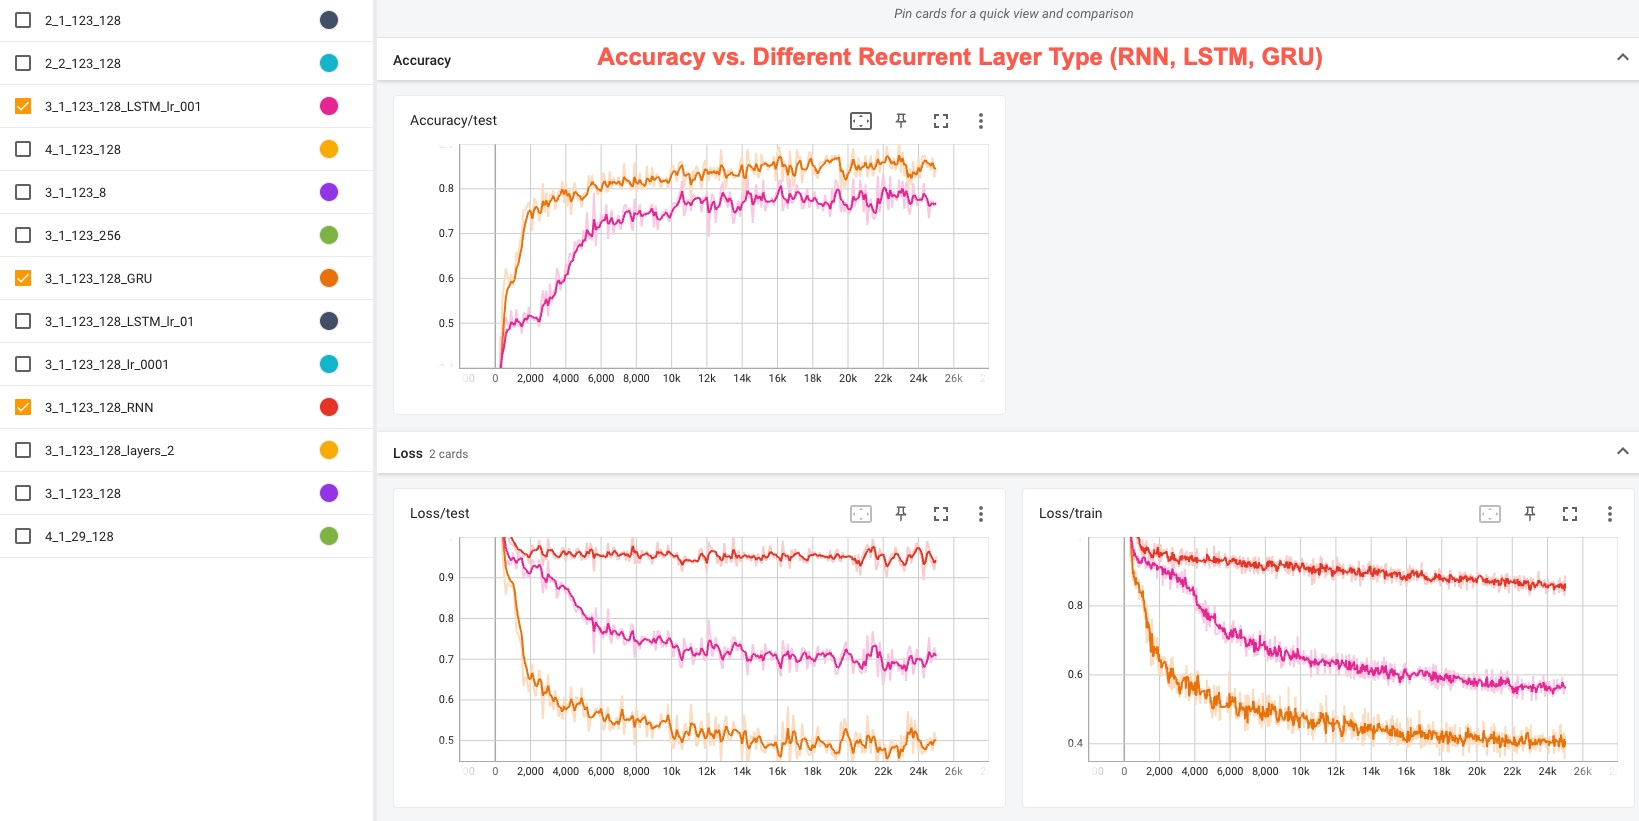
\includegraphics[width=16cm]{figures/hp_model_arch.jpg}
    
    \item Size of hidden state: Increasing the size of hidden state would improve model performance. However, this would come with at the cost of a larger model size and higher memory requirements
    
    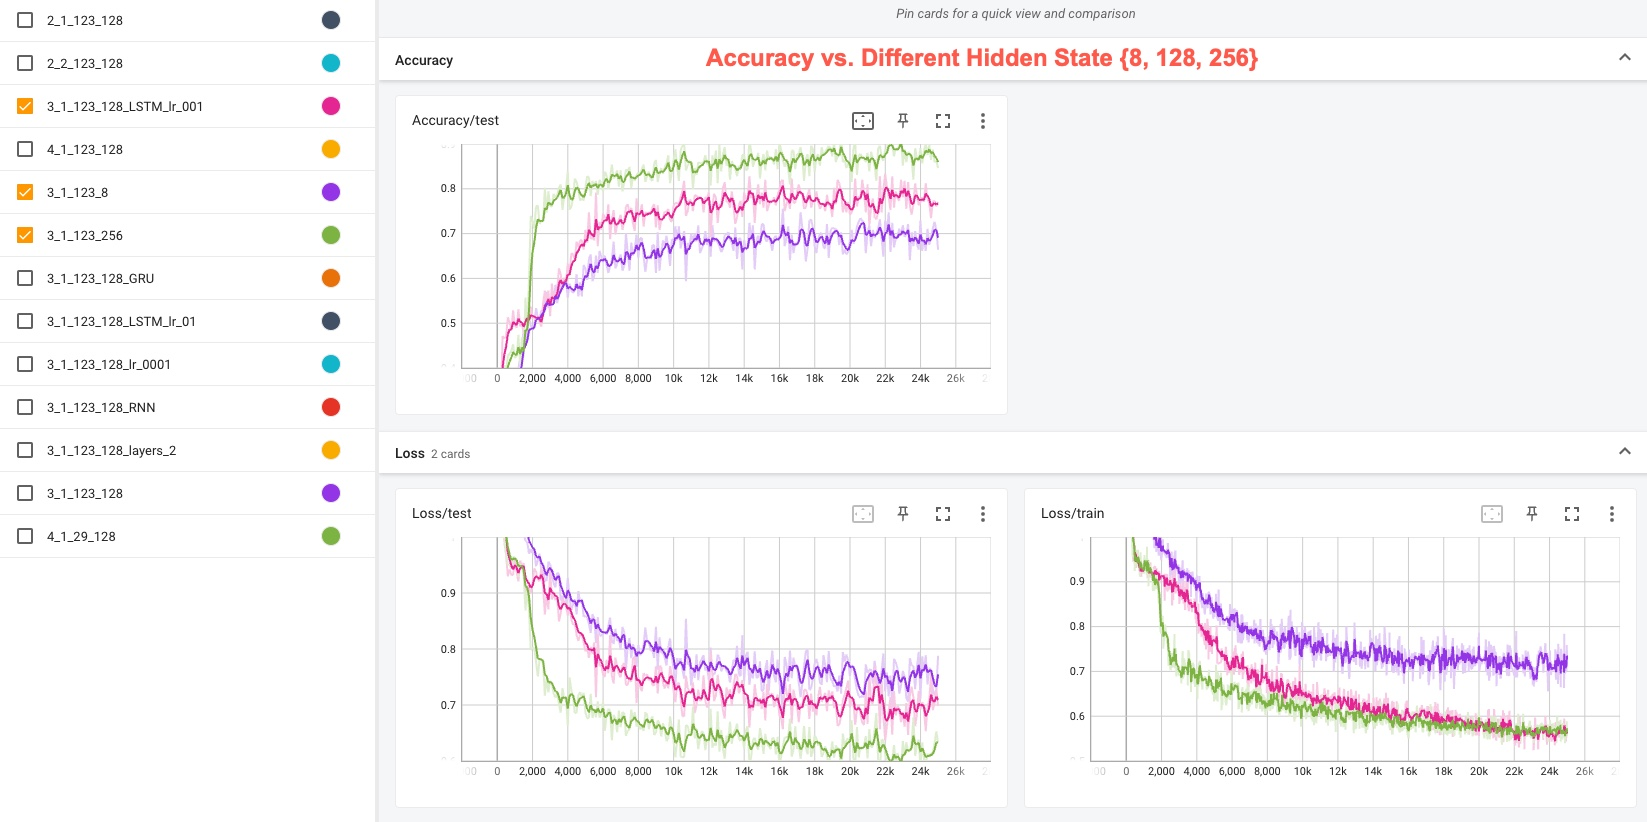
\includegraphics[width=16cm]{figures/hp_hidden_dim.jpg}
    
    \item Learning rate: Increasing the learning rate would quicken the convergence to the optimum weights. However the variance once the model has converged is higher. 

    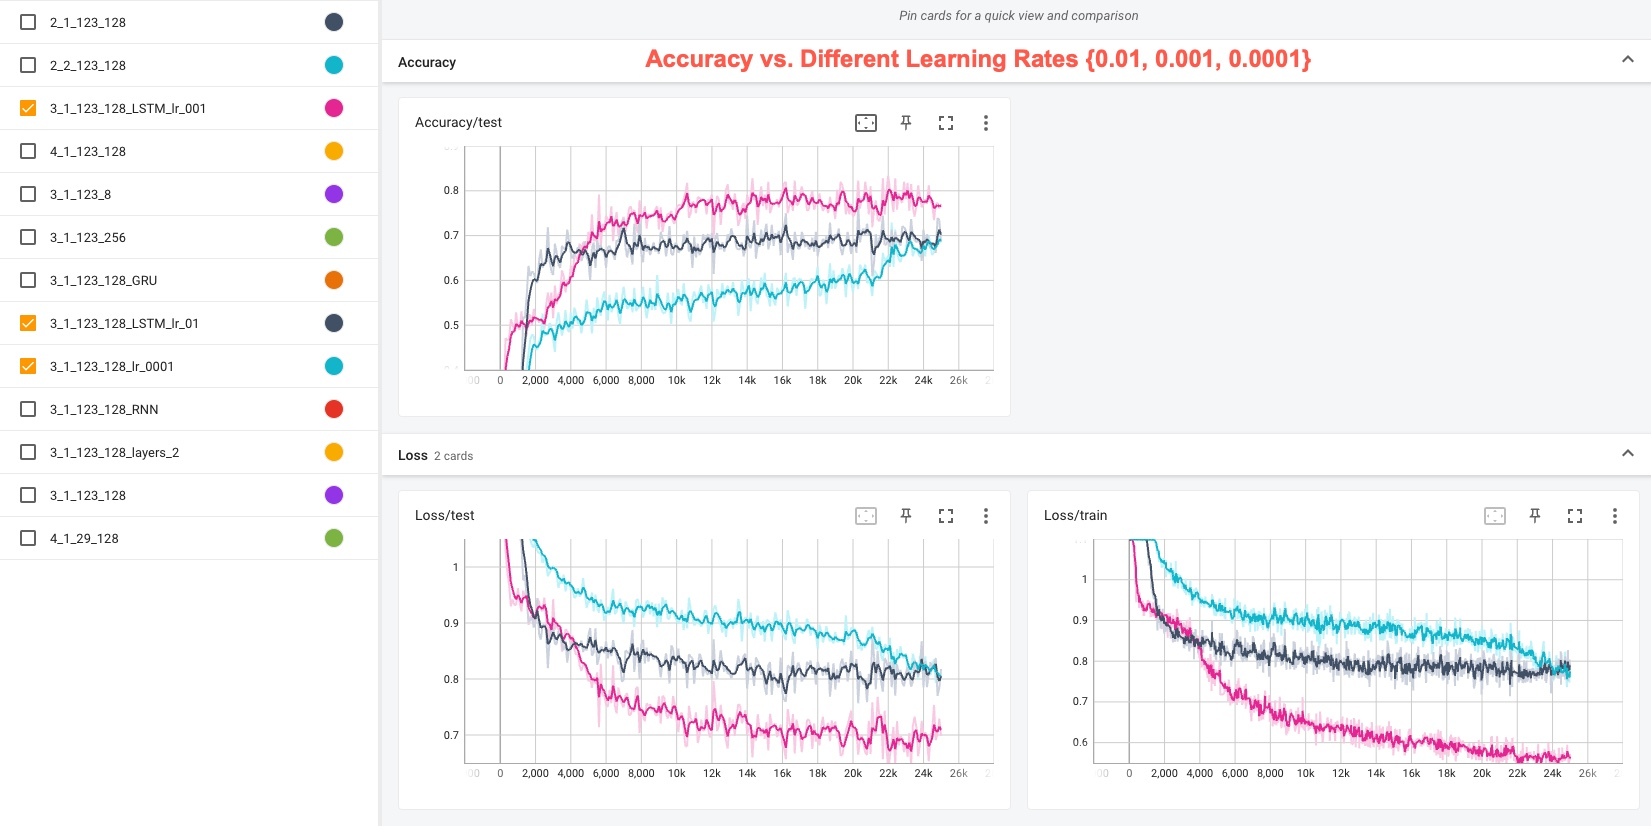
\includegraphics[width=16cm]{figures/hp_lr.jpg}
    
    \item Number of layers: A model with higher number of layers would generally yield higher accuracy. 

    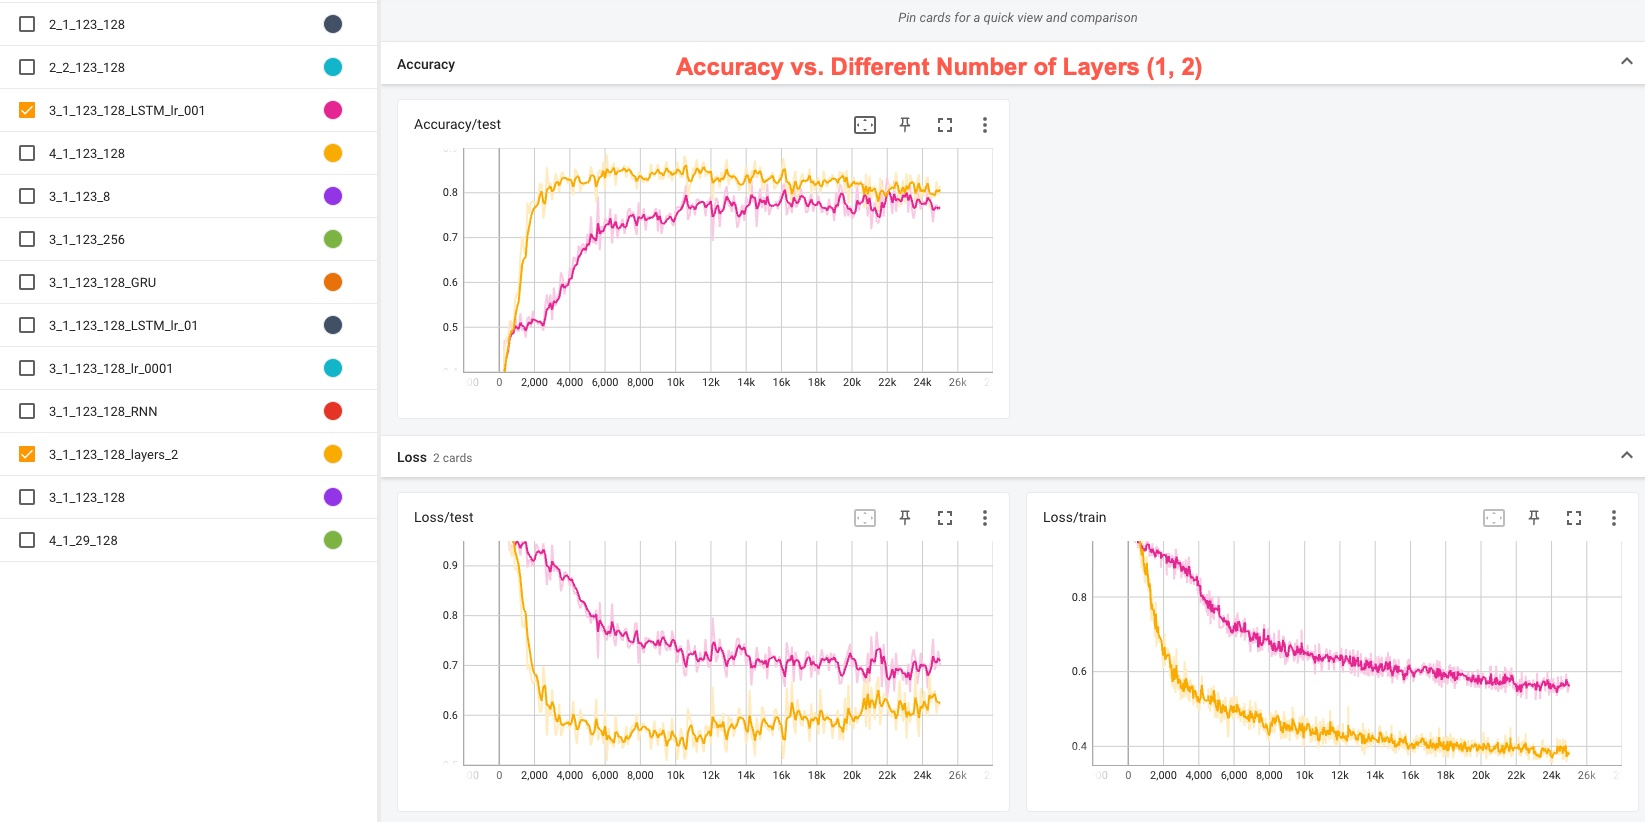
\includegraphics[width=16cm]{figures/hp_layers.jpg}
    
\end{itemize}


\end{answer}
% <SCPD_SUBMISSION_TAG>_4_a

\clearpage

\LARGE
4.b
\normalsize

% <SCPD_SUBMISSION_TAG>_4_b
\begin{answer}
Increasing the memory capacity improves the model performance (i.e., the accuracy on the meta-test query set) and likewise, decreasing the memory capacity deteriorates the model performance. The converged accuracy for $h = 8$ is less than the converged accuracy for $h=128$ which in turn is less than the converged accuracy for $h=256$.

$h$ is a model hyper-parameter which corresponds to the number of hidden states. A model with higher number of hidden states can represent the information contained within the support set better and more accurately, which in turn is used to make predictions on the test dataset.

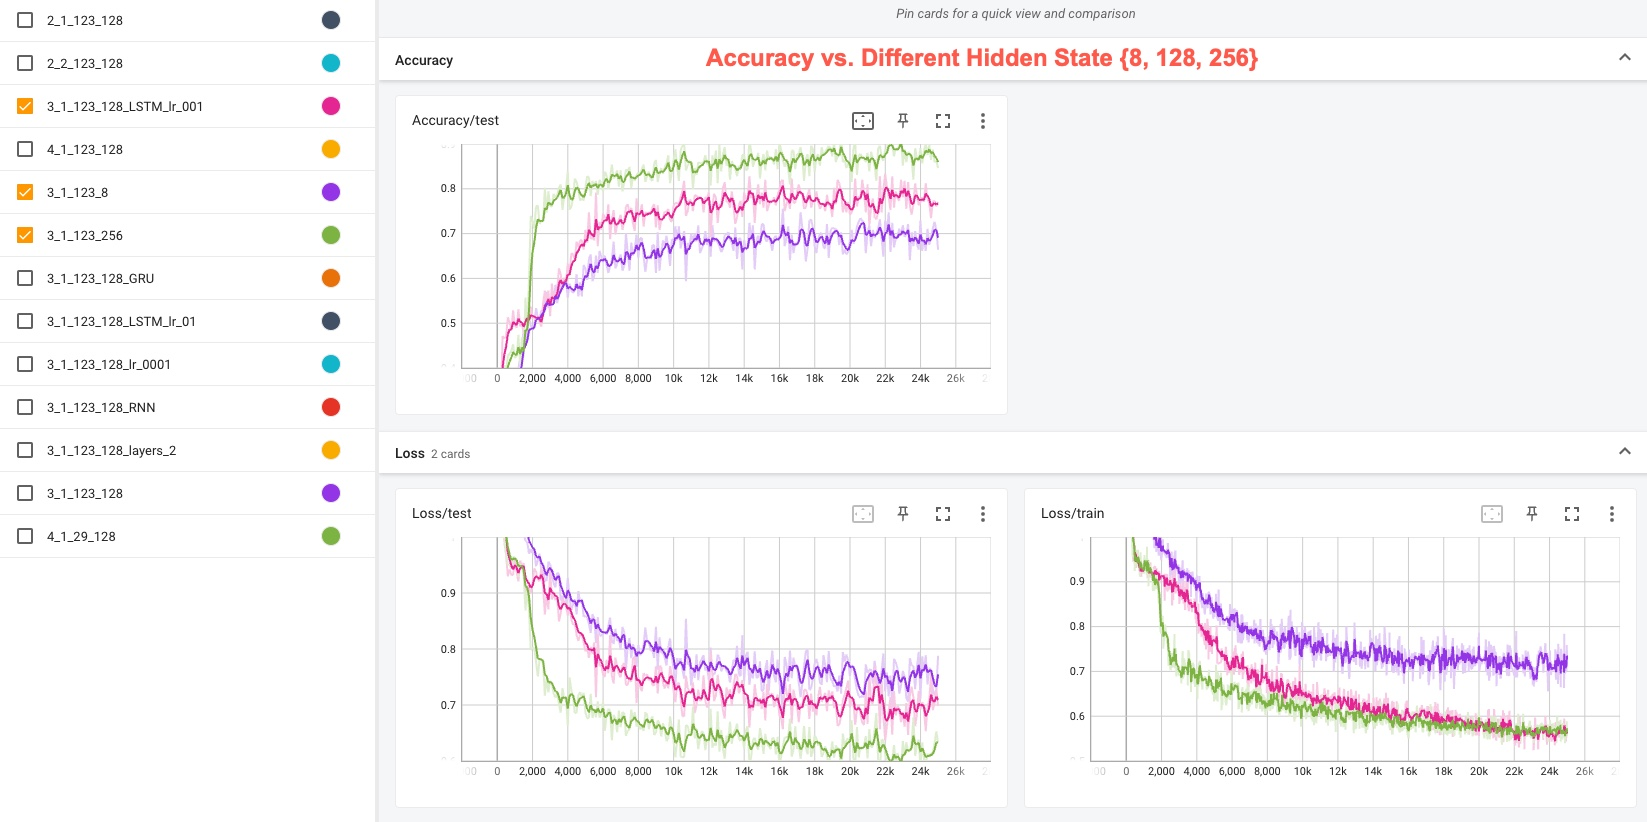
\includegraphics[width=16cm]{figures/hp_hidden_dim.jpg}

  \end{answer}
% <SCPD_SUBMISSION_TAG>_4_b

% <SCPD_SUBMISSION_TAG>_entire_submission

\end{document}